\section{Field-Programmable Gate Arrays}
\label{bg:sec:fpga}

\subsection{Computing Architectures}
\label{bg:sub:computing_architectures}

When it comes to implementing computations, we often choose from a spectrum of
computing machines.  These choices range from ones with fixed architectures
that computes by executing \emph{software} designs, such as \glspl{cpu} and
\glspl{gpu}, to ones that can implement custom \emph{hardware} architectures,
such as \glspl{fpga} and \glspl{asic}.

There has been a great amount of efforts in recent decades to make
fixed-architecture machines run as fast as possible; many novel and intricate
ideas were proposed and we now have a variety of general circuitries in
\glspl{cpu} to improve their performance~\cite{comparch}.  For instance,
\glspl{cpu} could have a pipeline that spans several clock cycles to fetch and
decode instructions, and access data from memory or registers to carry out
computations.  At the same time, they would make predictions about the branches
taken in control-flows, as the pipeline must be flushed if an incorrect
instruction is fetched, incurring a penalty in speed.  Superscalar architecture
and out-of-order execution are used to increase instruction-level parallelism.
They also exploit data-level and thread-level parallelism, in order to maximize
opportunities to parallelize computations.  These are just the tip of the
iceberg, as many other architectural advancements exist.

The great majority of fixed-architecture computing machines are based on
\emph{von Neumann architecture}, which consists of three parts: a computation
unit, a memory and a bus between them to move data back and forth.  Often
applications running on these machines could spend a majority of their time
and energy to move data and instructions in the memory from/to the right
location in the processor as fast as possible, in order to carry out arithmetic
computations.  Because computational tasks frequently reuse input data and
intermediate results, a hierarchy of caches, in tandem with cache-aware
compiler optimizations~\cite{kowarschik03}, are often used to mitigate the
costs of exchanging data between the processor and the memory.  Despite
these optimization efforts to run software code as fast as possible, the
processor-memory bus, which is often referred to as the \emph{von Neumann
bottleneck}~\cite{backus78}, inherently exist and it remains the limiting
factor of performance in the architecture, and this phenomenon is known to many
as \emph{hitting the memory wall}~\cite{bacon13, wulf94}.

Custom architectures in general achieve much higher performance, thanks to
their ability to implement arbitrary digital circuits specifically designed
for the application under consideration, and spatially distribute memory
bandwidth and computations.  This is in stark contrast to microprocessors
such as \glspl{cpu} and \glspl{gpu}, which utilize general-purpose circuitry
to cope with a wide-range of applications. \glspl{asic} provide the best
power efficiency and performance among all above architectures, however
they are often associated with long development cycles and high costs; any
updates to the design would require a complete and expensive re-spinning
of the circuits~\cite{bacon13}, as they are inherently non-programmable.
\Glspl{fpga} provide the best trade-off between processors and \glspl{asic}.
Not only do \glspl{fpga} have better performance and power characteristics
than fixed architectures, they also offer high programmability which makes
\glspl{fpga} cost-effective low-volume \gls{asic} replacements~\cite{karen04,
bacon13}.  At the same time, with a much shorter development period than
\glspl{asic}, a hardware design on \glspl{fpga} can be implemented with a much
lower cost.  With a shorter time to market, it further enables a substantially
larger profit by a competitively early market entry~\cite{semico12}.  For
the above reasons, being able to leverage parallelism from bit-level all the
way to the loop- and task-level, \glspl{fpga} have been increasingly used as
high-performance and low-power alternatives to \glspl{cpu} and \glspl{gpu}
for many classes of applications~\cite{bacon13, brodtkorb10, sirowy08}.  For
example, Thomas~\etal~\cite{thomas09} reported a \gls{fpga}-based random number
generator can obtain a $260\times$ speed-up, while costing less than 1\% of
energy to produce each random sample, when compared to its software counterpart
running on a \gls{cpu}\@.  Microsoft initiated a mid-scale deployment of
Stratix V \glspl{fpga} in their data center, improving the throughput of their
Bing web search engine by a factor of 95\%~\cite{catapult}.


\subsection{FPGA Architecture}
\label{bg:sub:fpga_architecture}

\Glspl{fpga} owe their high performance and power efficiency to the design of
the architecture, we thus use Altera Stratix V~\cite{stratix5} as an example to
explain the architecture.  Stratix V fabric contains a two-dimensional array of
\glspl{lab}.  Each \gls{lab} in turn consists of an array of 10 \glspl{alm}.
Figure~\ref{bg:fig:alm} shows a high-level block diagram of an \gls{alm} in
Stratix V.  In an \gls{alm}, multiplexers can be configured to choose whether
full adders and registers are used.  Dedicated full adders enable more complex
boolean functions to be implemented in a single \gls{alm}, whereas the use of
registers, which store intermediate values, determines whether the circuit
is combinational or sequential.  The two \glspl{lut} in an \gls{alm} can be
configured to compute a combination of two arbitrary boolean functions, each
with up to 5 inputs from 8 inputs in total.  Stratix 10, slated to be released
in the next couple of years, has up to 1.87 million \glspl{alm} and 7.47
registers in total for the most demanding applications~\cite{stratix10stat}.
Interconnects, another class of key configurable resources on \glspl{fpga},
enable the inputs and outputs of \glspl{alm} to be wired, in order to form
larger and complete circuits from the two-dimensional array of \glspl{alm}.
This allows the \gls{fpga} fabric to realize arbitrary digital circuits.
\begin{figure}[ht]
    \centering
    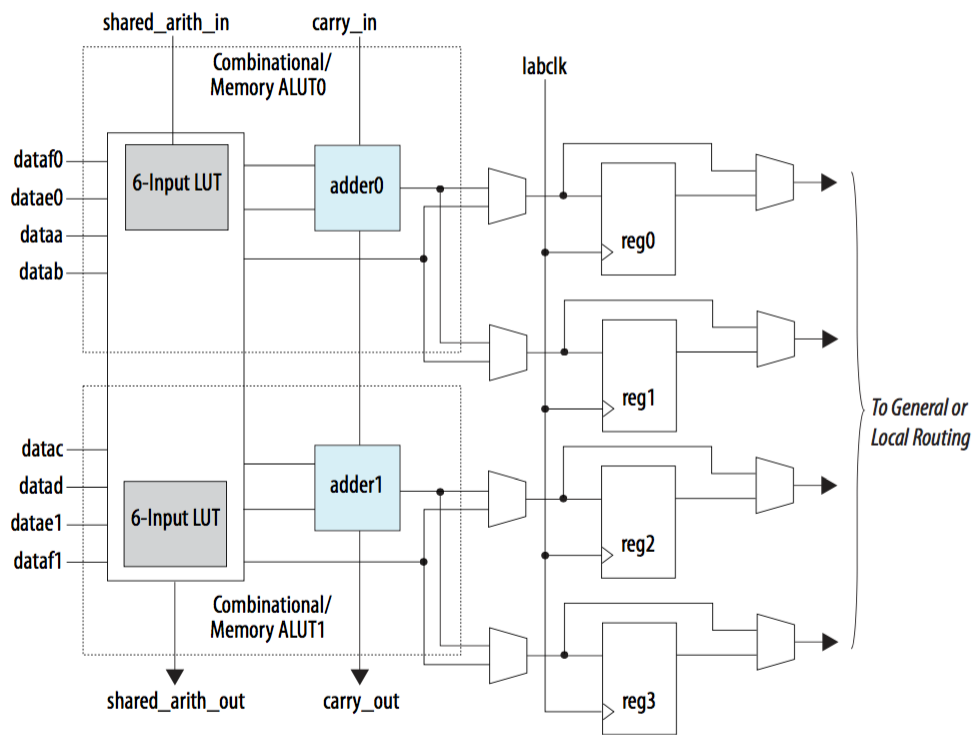
\includegraphics[width=0.8\linewidth]{bg/fig/alm.png}
    \caption{%
        A high-level block diagram of an \gls{alm} in Stratix V, from Stratix V
        Device Handbook~\cite{stratix5}.
    }\label{bg:fig:alm}
\end{figure}

% distributed memory and dsp elements

\Glspl{fpga} with enough \glspl{alm} and interconnects can implement arbitrary
digital designs.  This versatile architecture therefore overcomes the memory
wall problem by not restricting itself to von Neumann architecture.  As we have
mentioned earlier, \glspl{fpga} can implement a circuit that is individually
tailored for the application, in contrary, \glspl{cpu} have general-purpose
circuitries designed for a wide range of applications, which may therefore have
lower power-efficiency and performance.  Moreover, unlike the \gls{cpu} which
only has a small set of registers, the \gls{fpga} with its flexibility and
abundant registers, allows designs to distribute memory blocks and computation
units and place them in close proximity.

Traditionally, multipliers, when implemented as soft-logic in \glspl{fpga},
cost a large number of \glspl{alm}.  Stratix devices thus further include an
array of hardened components to carry out arithmetic operations distributed
on the \gls{fpga} fabric, known as \glspl{dsp} blocks, or simply \glspl{dsp}.
Because of the dedicated hardened circuits, \glspl{dsp} compute faster than
arithmetic operators formed by \glspl{alm} only, meanwhile they free \gls{alm}
resources to perform more non-arithmetic computations.  In Stratix V, each
variable-precision \gls{dsp} is paired with a \gls{lab}\@.  These \glspl{dsp},
can be configured in combinations to perform a wide variety of arithmetic
operations, ranging from using a single \gls{dsp} element to synthesize
three multipliers with two 9-bit inputs, up to combining four \glspl{dsp}
to form a complex-number multiplier with two 27-bit inputs~\cite{stratix5}.
Computations with larger inputs can also be implemented by using \glspl{alm}
and \glspl{dsp} to form larger arithmetic circuits.  Finally, Stratix 10 will
introduce hardened floating-point \glspl{dsp}, enabling IEEE 754~\cite{ieee754}
single-precision floating-point additions and multiplications, achieving a
performance of up to 10 \glspl{tflops}~\cite{stratix10fp}.  These \gls{dsp}
blocks can also be adapted to multiply fixed-point inputs.

\Glspl{dsp} accelerate arithmetic computations, however they need to be
supplied with inputs as fast as they can process to fully utilize them.
In general, in most applications, data are frequently reused by the same
computation unit.  Stratix V therefore include dedicated embedded memory called
M20K blocks (20 Kb storage) that can be arranged and combined into dual-port
\glspl{ram}.  Half of the \glspl{lab} on the device, called \glspl{mlab} can
also be configured to become a 640-bit \glspl{ram}.  These memory blocks are
distributed across the \gls{fpga} fabric, so that \glspl{dsp} can find them in
proximity.


\subsection{RTL Design Flow}
\label{bg:sub:rtl_design}

Modern \glspl{fpga}---with up to several million \glspl{lut}, and thousands
of embedded memory and \gls{dsp} blocks, wired through a programmable fabric
of interconnects---are humanly intractable to program at the granularity of
these individual components~\cite{kapre08}.  \Gls{fpga} applications are
thus commonly written in \gls{rtl} \gls{hdl}, such as Verilog~\cite{verilog}
and VHDL~\cite{vhdl}.  These \gls{hdl} source programs implement the desired
hardware by describing logics between registers.  \Gls{eda} tools can
then automatically translate these descriptions into hardware circuits in
\glspl{fpga}.

\Gls{eda} tools, go through several stages to synthesize \gls{hdl} source
code into circuits, To explain these stages in depth, we take Altera
Quartus II~\cite{quartus} as an example, which design flow is shown in
Figure~\ref{fig:quartus}.
\begin{figure}[ht]
    \centering
    \includegraphics[width=\textwidth]{bg/fig/quartus}
    \caption{Quartus II design flow.}\label{fig:quartus}
\end{figure}

Quartus II starts its compilation of the \gls{rtl} program by verifying
source code for syntax and semantic errors and design specification for
inconsistencies, then apply a methodology, called \emph{technology mapping},
which maps a topology of device-independent logic gates in logic expressions
onto a network of functional blocks (such as \glspl{lut}, \glspl{dsp}
and memory blocks) in the target \gls{fpga} device~\cite{cong08}; this
generated network is known as a \emph{technology-mapped netlist}.  In this
process, synthesis tools may optimize the circuit by performing additional
transformations such as redundant logic removal~\cite{quartus}.

The following stage, \emph{place \& route}, utilizes a heuristic placement
algorithm, which takes as it inputs the netlist, together with a device map
showing the location of each of its functional units, in order to select a
legal location on the \gls{fpga} for each functional block in the netlist,
such that the routing of these blocks is optimized~\cite{betz08}.  In general,
synthesis tools allow some freedom in the user's preference of the placement
of circuit.  Additional automated optimizations can be applied to improve
performance.  For example, Quartus II has the option to enable \emph{register
retiming}~\cite{quartus}, which allows registers to move across combinational
logic to reduce \emph{critical path} delay, \ie~the longest delay required
for an output of any source register to propagate to the input of any target
register in the circuit.  The end result of this step is a circuit schematic
on the target \gls{fpga}\@.  In the following step, the tool thus computes the
longest delay of all critical paths, which determines the maximum frequency at
which the application can run.  Users can also inspect the list of critical
paths and their delay statistics, so that one can focus their effort on
optimizing the timing of these critical paths by splitting it up by adding
registers, for instance.  The user can then choose to simulate the design using
\gls{eda} simulation tools.  Finally, the circuit generated by the tool can
be translated into a \emph{bitstream}, which is binary data that can be used
to program the \gls{fpga}\@.  Similar to processors, which can be programmed
by incrementally reading and executing instructions from an executable
program file, a bitstream is used to program the individual components such
as \glspl{lut}, \gls{dsp} blocks, dedicated memory blocks and interconnects
on an \gls{fpga}, so the circuit can be formed on the device.  The difference
between them is that while processors continuously read instructions from
memory, \glspl{fpga} are typically programed only once during the initial
setup, and the bitstream data are used spatially to infer a circuit rather than
sequentially as instructions~\cite{guccione08}.
